\chapter{Evaluation}\label{ch:eval}
\label{sec:eval:overall}

The project fulfilled all its success criteria and was successfully completed.

A large subset of Beam features were implemented in Elixir Dataflow~(\cref{sec:eval:limitations}).
A DSL was created which follows patterns native to Elixir.
It allows for low-impedance translation of a conceptual Dataflow Pipeline to its representation in code, achieving a dramatic reduction in code size over a Java version~(\cref{sec:eval:twitter:code}).

Elixir Dataflow displays performance superior to the optimised Apache Flink Beam runner, proving able to deal with busy streams of data and large Pipelines while displaying excellent latency characteristics and scalability~(\cref{sec:eval:latency}).
It has also been shown to work in real-world scenarios and is able to process a stream of $\sim$\num{25000} tweets per second, driving a hashtag autocompletion algorithm.

The project weighs in at approximately \num{3200} lines of Elixir code (excluding comments, blank lines and tests).
Approximately \num{12000} lines of code were written over the lifetime of the project, illustrating the volatility of the codebase due to evolving requirements.

In comparison, the core Beam codebase comprises $\sim$\num{78000} lines of code, though it implements some functionality which is out-of-scope for the Elixir implementation.

\section{Feature analysis}\label{sec:eval:limitations}

The Beam Capability Matrix~\cite{Beam-Cap-Matrix} is a standard method of feature comparison among Beam implementations.
\Cref{tab:eval:capability} shows the Capability Matrix augmented with a column indicating features implemented during this project.

\newcommand{\pmark}{$\sim$}
\begin{table}
	\caption[Apache Beam Capability Matrix including the Elixir implementation.]{The Capability Matrix~\cite{Beam-Cap-Matrix} compares support for Beam Model features across implementations. The~\pmark~symbol indicates a partial implementation.}
	\label{tab:eval:capability}	
	\tabulinesep=1.4mm
	\begin{tabu}{|X[2.8,r,m]|X[c,m]|X[c,m]|X[c,m]|X[c,m]|X[c,m]|} \firsthline
		& \textbf{Beam Model} & \textbf{Google Cloud Dataflow} & \textbf{Apache Flink} & \textbf{Apache Spark} & \textbf{Elixir Dataflow} \\ \hline\hline
		
		\multicolumn6{|c|}{\textbf{What is being computed?}} \\ \hline
		%\tabuphantomline
		ParDo & \cmark & \cmark & \cmark & \cmark & \cmark \\ \hline
		GroupByKey & \cmark & \cmark & \cmark & \pmark & \cmark \\ \hline
		Flatten & \cmark & \cmark & \cmark & \cmark & \xmark \\ \hline
		Combine & \cmark & \cmark & \cmark & \cmark & \cmark \\ \hline
		Composite Transforms & \cmark & \pmark & \pmark & \pmark & \pmark \\ \hline
		Side Inputs & \cmark & \cmark & \cmark & \cmark & \xmark \\ \hline
		Source API & \cmark & \cmark & \cmark & \cmark & \xmark \\ \hline
		Aggregators & \pmark & \pmark & \pmark & \pmark & \xmark \\ \hline
		Stateful processing & \cmark & \pmark & \pmark & \xmark & \xmark \\ \hline\hline
		
		\multicolumn6{|c|}{\textbf{Where in event-time?}} \\ \hline
		Global windows & \cmark & \cmark & \cmark & \cmark & \cmark \\ \hline
		Fixed windows & \cmark & \cmark & \cmark & \cmark & \cmark \\ \hline
		Sliding windows & \cmark & \cmark & \cmark & \cmark & \cmark \\ \hline
		Session windows & \cmark & \cmark & \cmark & \cmark & \pmark \\ \hline
		Custom windows & \cmark & \cmark & \cmark & \cmark & \cmark \\ \hline
		Custom merging windows & \cmark & \cmark & \cmark & \cmark & \pmark \\ \hline
		Timestamp control & \cmark & \cmark & \cmark & \cmark & \cmark \\ \hline
		Watermark domains & \xmark & \xmark & \xmark & \xmark & \cmark \\ \hline \hline
		
		\multicolumn6{|c|}{\textbf{When in processing-time?}} \\ \hline
		Configurable triggering & \cmark & \cmark & \cmark & \xmark & \cmark \\ \hline
		Event-time triggers & \cmark & \cmark & \cmark & \xmark & \cmark \\ \hline
		Processing-time triggers & \cmark & \cmark & \cmark & \cmark & \xmark \\ \hline
		Count triggers & \cmark & \cmark & \cmark & \xmark & \pmark \\ \hline
		(Meta)data-driven triggers & \xmark & \xmark & \xmark & \xmark & \xmark \\ \hline
		Composite triggers & \cmark & \cmark & \cmark & \xmark & \pmark \\ \hline
		Allowed lateness & \cmark & \cmark & \cmark & \xmark & \cmark \\ \hline
		Timers & \cmark & \pmark & \pmark & \xmark & \pmark \\ \hline \hline
		
		\multicolumn6{|c|}{\textbf{How do refinements relate?}} \\ \hline
		Discarding mode & \cmark & \cmark & \cmark & \cmark & \cmark \\ \hline
		Accumulating mode & \cmark & \cmark & \cmark & \xmark & \cmark \\ \hline
		Retractions & \xmark & \xmark & \xmark & \xmark & \xmark \\ \lasthline
	\end{tabu}
\end{table}

As the Matrix demonstrates, no implementation is feature-complete in spite of Beam containing core Java classes to be used as the basis for feature implementation---something this project could not take advantage of.
Over the course of this Part~II project, a significant amount of features were implemented.
The features omitted, such as Side Inputs, Sources and Aggregators, were ones which would require a lot of code support but focused on ancillary functions rather than the core Model.
The only limitation not shown in \cref{tab:eval:capability} is the lack of support for non-linear Pipelines.

Some core modules were implemented using na\"ive algorithms to save time.
For instance, a linear list-based priority queue was used in several grouping and windowing algorithms.
In spite of this, the performance of the implementation was excellent, as the rest of this chapter shows.

\section{Approach to empirical evaluation}\label{sec:eval:approach}

\subsection{Test environment}\label{sec:eval:approach:environment}

Efforts were made to collect data in a consistent environment to reduce the chance of unwanted variation.

All tests were conducted on a MacBook Pro (15-inch, Late 2016) with a \SI{2.9}{\giga\hertz} Intel Core~i7 CPU and \SI{16}{GB} of \SI{2133}{\mega\hertz} RAM running macOS 10.12.4.
Runtimes used were Elixir 1.4.2 on OTP 19 and the Oracle JRE v1.8.0\_66-b17.
Apache Beam v0.7.0 was used in the experiments.

Prior to conducting the tests, all non-essential background processes and applications were terminated.
Tests were initiated using a scripted test runner in order to replicate multiple instances of the tests accurately.

\subsection{Data collection and processing methodologies}\label{sec:eval:approach:collection}

A custom test runner was developed in Elixir for the purpose of scheduling and running experiments.
It was configured with tests for both Java and Elixir implementations.
Each test was executed via a new system process with configuration passed as command-line arguments.
A new VM instance was spawned each time for both Elixir and Java tests to maintain consistency and accuracy.

The test runner measured CPU and memory usage of the spawned process using the \verb|ps| utility.
Other measurements, such as latency, were recorded directly by the instrumented binary.

The data were then processed, analysed and plotted using MATLAB.

\section{The Twitter Pipeline}\label{sec:eval:approach:twitter}

Twitter is a popular social network focused on posting short messages, or \emph{tweets}.
Tweets tend to include \emph{hashtags}, words or short phrases preceded by the \# character.
Hashtags rely on many users using the exact hashtag text in their tweets.
The hashtag can then be used to aggregate and list all of these tweets, perhaps all on a particular topic.

An autocomplete feature would be useful when composing tweets to suggest popular hashtags and discourage misspellings.
This real-world scenario formed the basis of an evaluation exercise.

Twitter's free streaming API~\cite{TwitterStreamingAPI} was used to receive a stream of English-language tweets.
Thirteen search terms pertaining to technology (such as `tech' and `Google') were passed to the API to constrain the results.

It is beneficial to have autocompletion data which is as up-to-date as possible, but equally, it is important to take into account older data.
Therefore, the tweets were windowed into sliding windows with size \SI{3}{\min} and period \SI{1}{\min}.
This meant that an up-to-date autocompletion list was emitted every \SI{1}{\min}.
Each of these was derived from tweets seen in the preceding \SI{3}{\min}.

\Cref{fig:eval:twitter-pipeline-dag} illustrates the Pipeline used to process the tweets.
In a real web application, the results would be sent to another process or published to a message broker in order to enable a web server to handle user requests for autocompletion suggestions.
For the purposes of this experiment they were logged to the console.

\begin{figure}
	\centering
	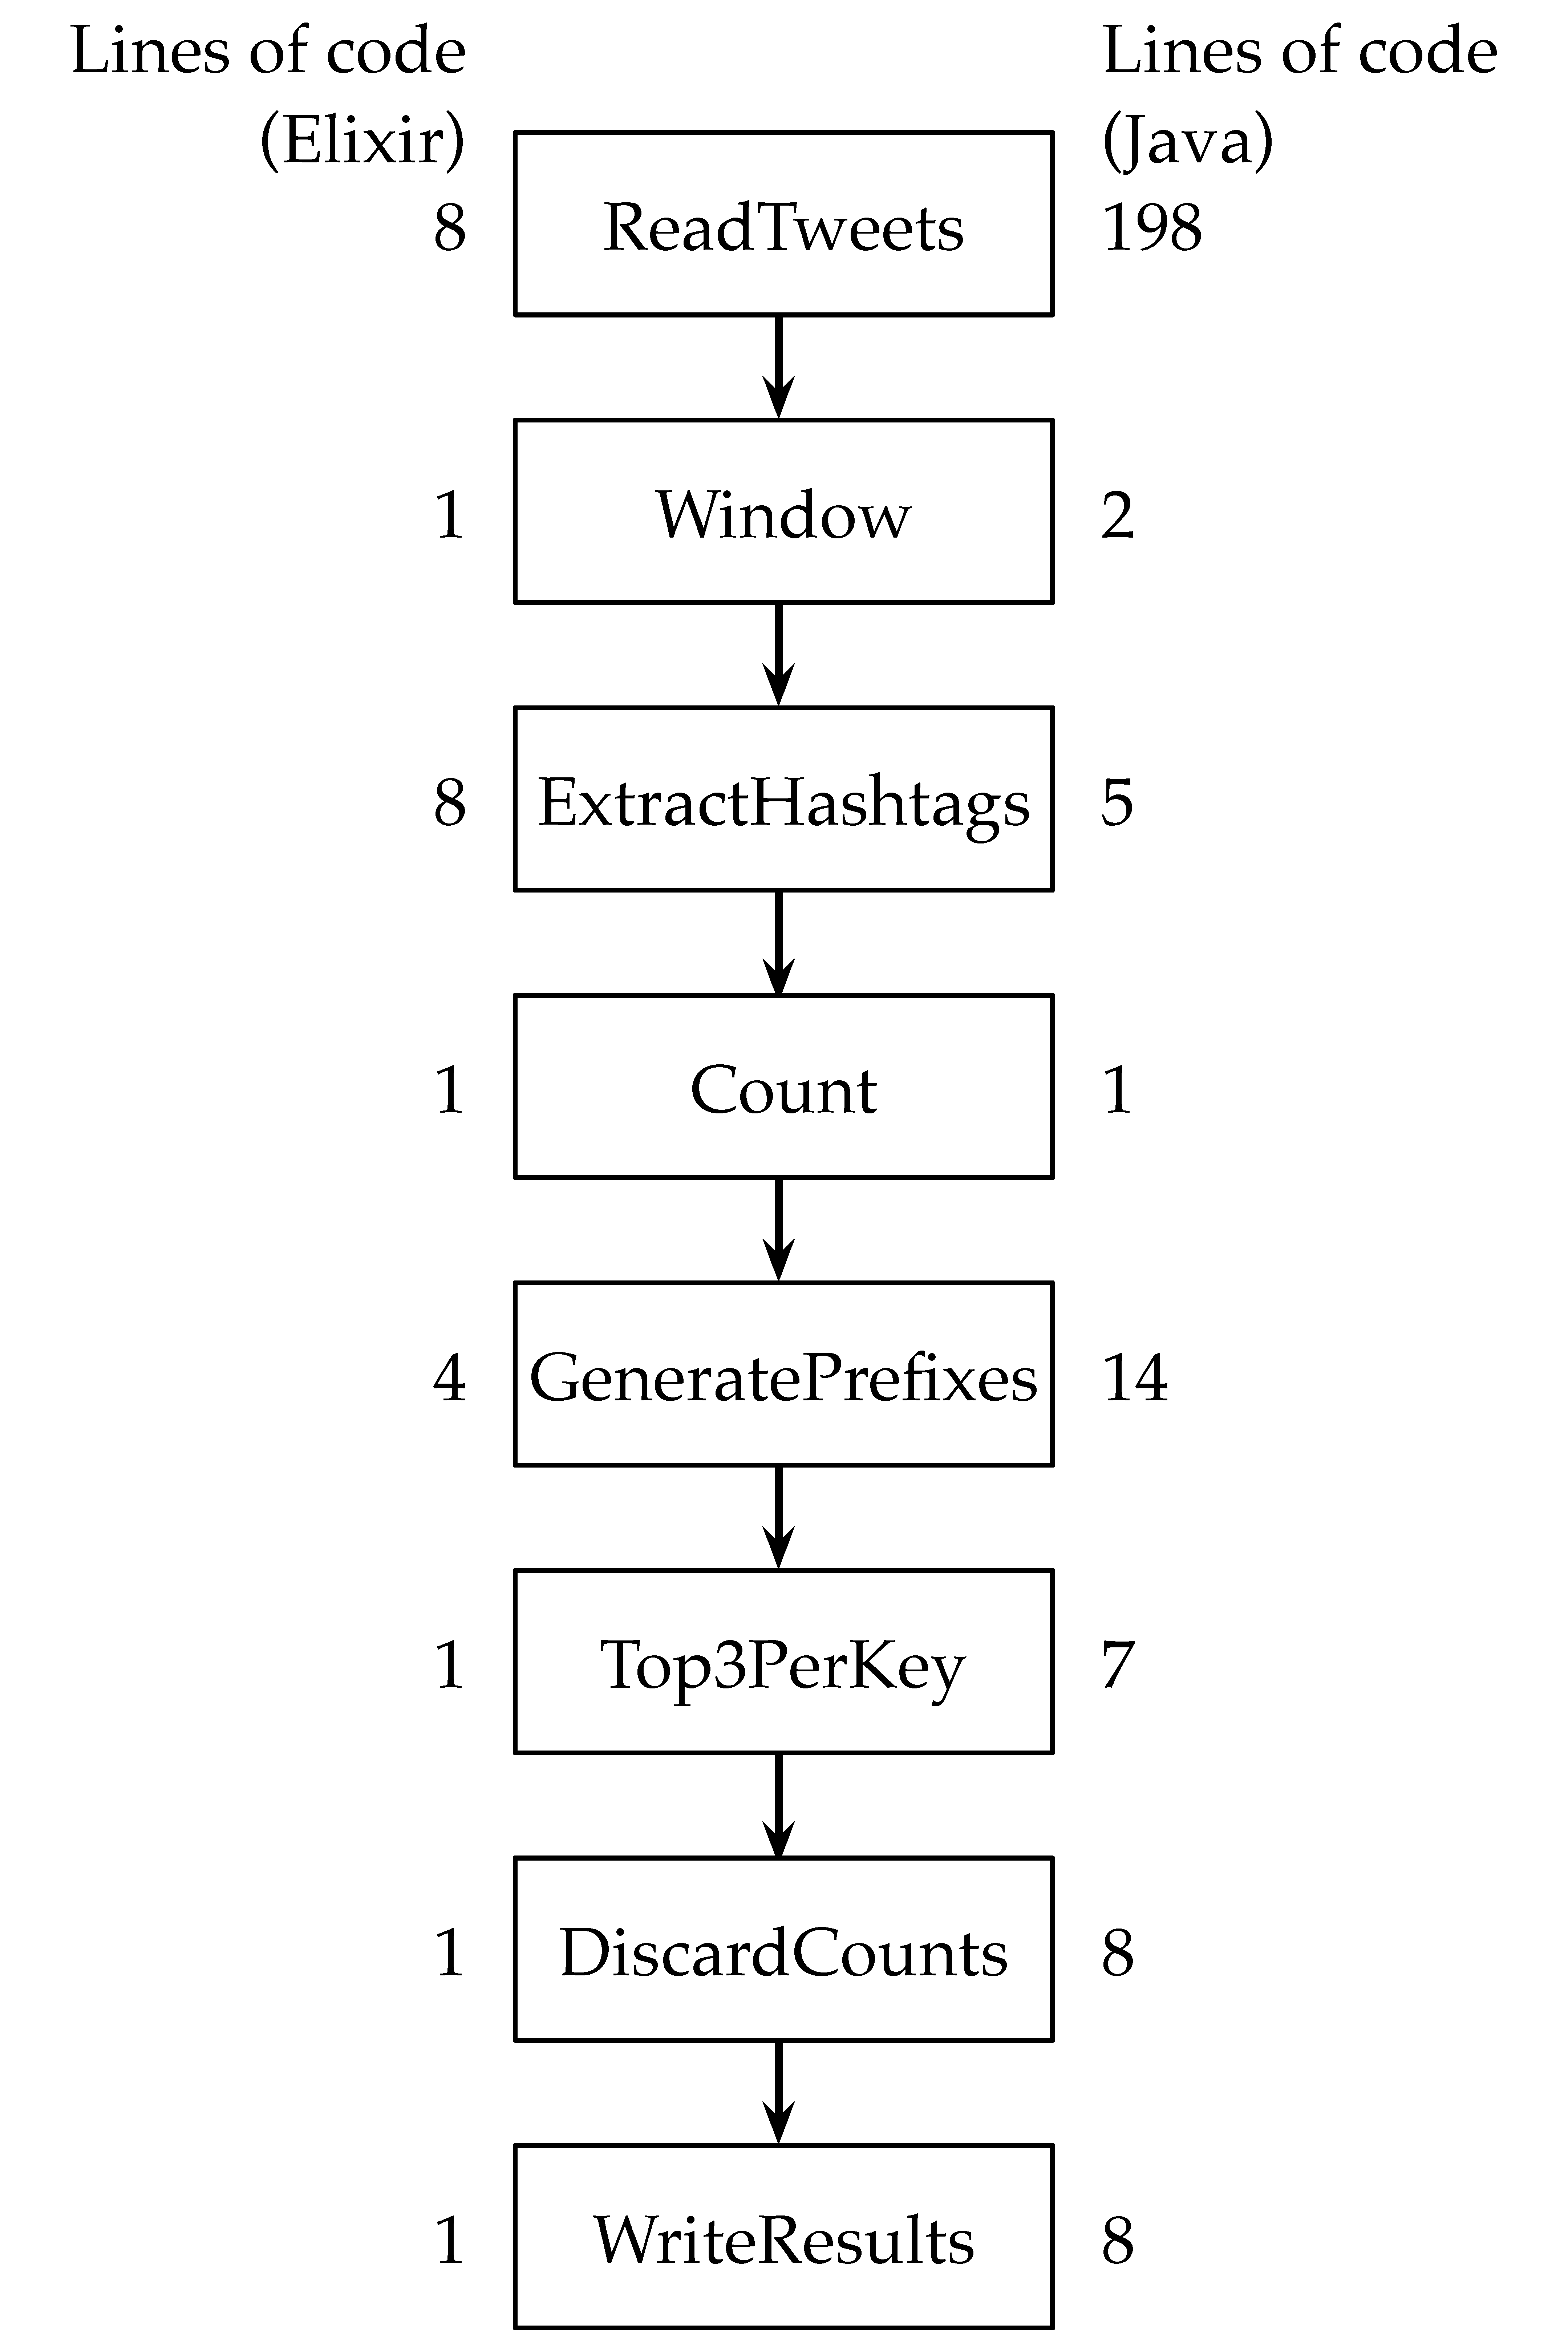
\includegraphics[height=0.6\textheight]{images/diags/eval-twitter-pipeline}
	\caption[The Twitter Pipeline as a Directed Acyclic Graph.]{The Twitter experiment uses a Pipeline representative of a real-world application. The lines-of-code needed to implement each step in the Pipeline are also shown.}
	\label{fig:eval:twitter-pipeline-dag}
\end{figure}


The scenario provides a good way to test various features of the Model.
Sliding windowing is used, and multiple stages of aggregation are employed.
The Pipeline utilises both Elementwise and Grouping Transforms.

The free stream provided by Twitter delivers \num{40}--\num{70} tweets per second, up to \SI{1}{\percent} of the Firehose ($\sim$\num{7000} tweets per second).
Over the execution of the experiment, an average rate of \num{50} tweets per second was observed.
To simulate a larger stream and evaluate the throughput of the runner, a configurable way to replicate each tweet by a multiplicative factor was added.

The ability to keep up with the stream and be able to output a batch of data derived from the preceding \SI{3}{\min} every \SI{1}{\min} indicates success in the experiment.

The next section explores the programmer-facing differences when implementing this Pipeline in Elixir and Java.
\Cref{sec:eval:twitter:throughput} evaluates the throughput abilities of the Elixir runner.
The Beam DirectRunner was not evaluated as it could not keep up with the stream even without expansion.
Its limits are discussed in \cref{sec:eval:latency}.

\subsection{Code comparison}\label{sec:eval:twitter:code}

The Pipeline was implemented in both Java (Beam) and Elixir.
The full code is available in \cref{apx:twitter-code}; what follows is a comparison of selected excerpts which illustrate differences between the two.

The Java code is noticeably longer, requiring 220 lines of code (excluding blank lines and comments) compared to the 35 lines required in Elixir.

\begin{codelisting}
	\caption{Reading a Twitter stream as an unbounded source in Elixir.}
	\label{lst:eval:twitter-readstream-elixir}
	\begin{minted}[breaklines=true]{elixir}
parse_as_timestamp = fn string ->
  string
  |> Timex.parse!("{WDshort} {Mshort} {0D} {h24}:{0m}:{0s} {Z} {YYYY}")
  |> DateTime.to_unix
  |> DTime.timestamp(:seconds)
end
terms = [...]
#...
p
~> "Read Stream" -- IO.read_stream(fn -> ExTwitter.stream_filter(track: terms, language: "en") end)
~> "Extract Timestamps" -- Windowing.with_timestamps(&parse_as_timestamp.(&1.created_at),
     delay_watermark: {30, :seconds, :event_time})
# `&parse_as_timestamp.(&1.created_at)` is captured lambda syntax for
# fn tweet -> parse_as_timestamp.(tweet.created_at) end
	\end{minted}
\end{codelisting}

\begin{codelisting}
	\caption[Reading a Twitter stream as an unbounded source in Java.]{Reading a Twitter stream as an unbounded source in Java. Code compressed for readability, the full version~(\cref{lst:apxb:twitter-java}) is 194 LoC.}
	\label{lst:eval:twitter-readstream-java}
	\begin{minted}[breaklines=true]{java}
static class DummyCheckpoint
    implements UnboundedSource.CheckpointMark, Serializable { /*...*/ }
    
static class TwitterSource
    extends UnboundedSource<Status, DummyCheckpoint> {
    /*...*/
        
    @Override
    public UnboundedReader<Status> createReader(
        PipelineOptions options,
        @Nullable DummyCheckpoint checkpointMark
    ) throws IOException { /*...*/ }

    protected static class Reader
    extends UnboundedSource.UnboundedReader<Status>
    implements StatusListener {
        /*...*/
        private Reader(String[] terms, TwitterSource source) { /*...*/ }
        @Override public boolean start() throws IOException { /*...*/ }
        @Override public boolean advance() throws IOException { /*...*/ }
        @Override public Status getCurrent() throws NoSuchElementException { /*...*/ }
        @Override public Instant getCurrentTimestamp() throws NoSuchElementException { /*...*/ }
        @Override public void close() throws IOException { /*...*/ }
        @Override public Instant getWatermark() { /*...*/ }
        /*...*/
        @Override public void onStatus(Status status) { /*...*/ }
        /*...*/
    }
}
/*...*/
String[] terms = {/*...*/};

p.apply("GetTweets", Read.from(TwitterSource.withTerms(terms)))
	\end{minted}
\end{codelisting}

\subsubsection{Reading tweets}

One of the primary reasons for the length of the Java version is the necessary method of consuming the stream of tweets.

The Elixir standard library provides a way to deal with potentially unbounded, lazy data---\exs{Stream}s.
As such, it makes sense that one of the Root Transforms implemented in Elixir Dataflow is \exs{IO.read_stream}.

\Cref{lst:eval:twitter-readstream-elixir} illustrates this well.
\exs{ExTwitter} \cite{ExTwitter} is a Twiter client for Elixir, and it returns a standard \exs{Stream} when used to query the Twitter API.

In Elixir, the \exs{Windowing.with_timestamps} Transform provides a way to assign data-based timestamps to elements and generate a watermark based on a heuristic.
The emission of a watermark at this stage is only possible because of the watermark domains feature~(\cref{sec:impl:dataflow:watermark-generation}).
In this case, the output watermark is \SI{30}{\second} before the highest timestamp seen so far.
This means a tweet in the stream can be up to \SI{30}{\second} `out of order' before it causes lateness in the Pipeline.
This is important as the stream is not guaranteed to be ordered.

In Java, almost 200 lines of code are needed to read, timestamp and watermark the tweets~(\cref{lst:eval:twitter-readstream-java}).
The lack of a community standard for streams means that each data source needs to manage its own asynchronous logic.
For instance, \texttt{Twitter4J} \cite{Twitter4J} (the Twitter library used) requires the registration of a subscriber with callback methods.

In order to `connect' the Twitter stream to the Pipeline, an \texttt{UnboundedSource} (part of the Source API) had to be written.
The code listing shows the incidental complexity inherent in Java code, requiring implementation of massive interfaces even when only simple functionality is required.

The Source must manage its own timestamping and watermark generation and cannot use a standard Transform as in Elixir.
This leads to the tight coupling of the logic which reads, buffers and emits tweets obtained from the network with timestamp generation and watermarking logic.
Due to Java's concurrency model, thread-safety code needs to be included as well.

It is clear that Elixir's conventions around \exs{Stream}s and decoupled, modular design make it the superior solution in this case.

\subsubsection{Lambdas vs.\ classes}

The Dataflow Model adopts an intrinsically functional model of computation based on data transformations.
Java's support for this model is poor.
This is exemplified best by the need to specify logic in small internal classes as in \cref{lst:eval:twitter-lambdas-java}.
\Cref{lst:eval:twitter-lambdas-elixir} shows that Elixir, a functional language, excels at expressing these kinds of computation natively.

\begin{codelisting}
	\caption[Using internal classes to specify transformation logic in Java.]{In Java, there is often a need to use internal classes to specify logic. While Java~8 lambdas can be used, the lack of type inference means that internal classes are often a cleaner solution.}
	\label{lst:eval:twitter-lambdas-java}
	\begin{minted}[breaklines=true]{java}
 public static class GeneratePrefixesFn
 extends SimpleFunction<KV<String, Long>, List<KV<String, KV<String, Long>>>> {
    @Override
    public List<KV<String, KV<String, Long>>> apply(KV<String, Long> tagWithCount) {
        List<KV<String, KV<String, Long>>> result = new ArrayList<>();
        String downcased = tagWithCount.getKey().toLowerCase();
        for (int i = 1; i <= downcased.length(); i++) {
            String prefix = downcased.substring(0, i);
            result.add(KV.of(prefix, tagWithCount));
        }
     return result;
    }
}
public static class DiscardCountsFn
extends SimpleFunction<KV<String, List<KV<String, Long>>>, KV<String, List<String>>> {
    @Override
    public KV<String, List<String>> apply(KV<String, List<KV<String, Long>>> el) {
        List<String> prefixes = l.getValue().stream().map((KV::getKey)).collect(Collectors.toList());
        return KV.of(el.getKey(), prefixes);
    }
}
/*...*/
.apply("GeneratePrefixes", FlatMapElements.via(new GeneratePrefixesFn()))
/*...*/
.apply("DiscardCounts", MapElements.via(new DiscardCountsFn()))
	\end{minted}
\end{codelisting}

\begin{codelisting}
	\caption[Using lambdas to specify transformation logic in Elixir.]{The functional paradigm of Elixir enables the specification of transformation logic in an idiomatic manner.}
	\label{lst:eval:twitter-lambdas-elixir}
	\begin{minted}[breaklines=true]{elixir}
~> "Generate Prefixes" -- Core.flat_map(fn {tag, count} ->
  len = String.length tag
  for i <- 0..(len-1), downcased = String.downcase(tag),
    prefix = String.slice(downcased, 0..i),
    do: {prefix, {tag, count}}
 end)
# ...
~> "Discard Exact Counts" -- Core.map(fn {prefix, tcs} ->
  {prefix, Enum.map(tcs, fn {tag, _count} -> tag end)}
 end)
	\end{minted}
\end{codelisting}

\subsubsection{Summary}

Though formal user studies were not performed to assess the ease of use of the two SDKs empirically, the preceding examples show that Elixir as a language is much better suited to express the concepts of the Dataflow Model in code.

Java's paradigm is orthogonal to the way computation is reasoned about in the Model.
Even when a fluent API and Java~8 lambdas are employed, the lack of type inference buries the meaning of the code behind countless type annotations.

\subsection{Throughput evaluation}\label{sec:eval:twitter:throughput}

The Elixir Twitter Pipeline was executed with the multiplicative factor varying from \num1 to \num{10000}, i.e.\ approximately between \num{50} and \num{500000} tweets per second, in order to determine the maximal throughput of the Pipeline.
For comparison, the Twitter Firehose has an average tweet rate of \SI{7000}{\per\second}.
Each experiment was run for \SI{9}{\min}, allowing for \num9 discrete panes of output, spanning \num3 disjoint time intervals.

\begin{figure}
	\centering
	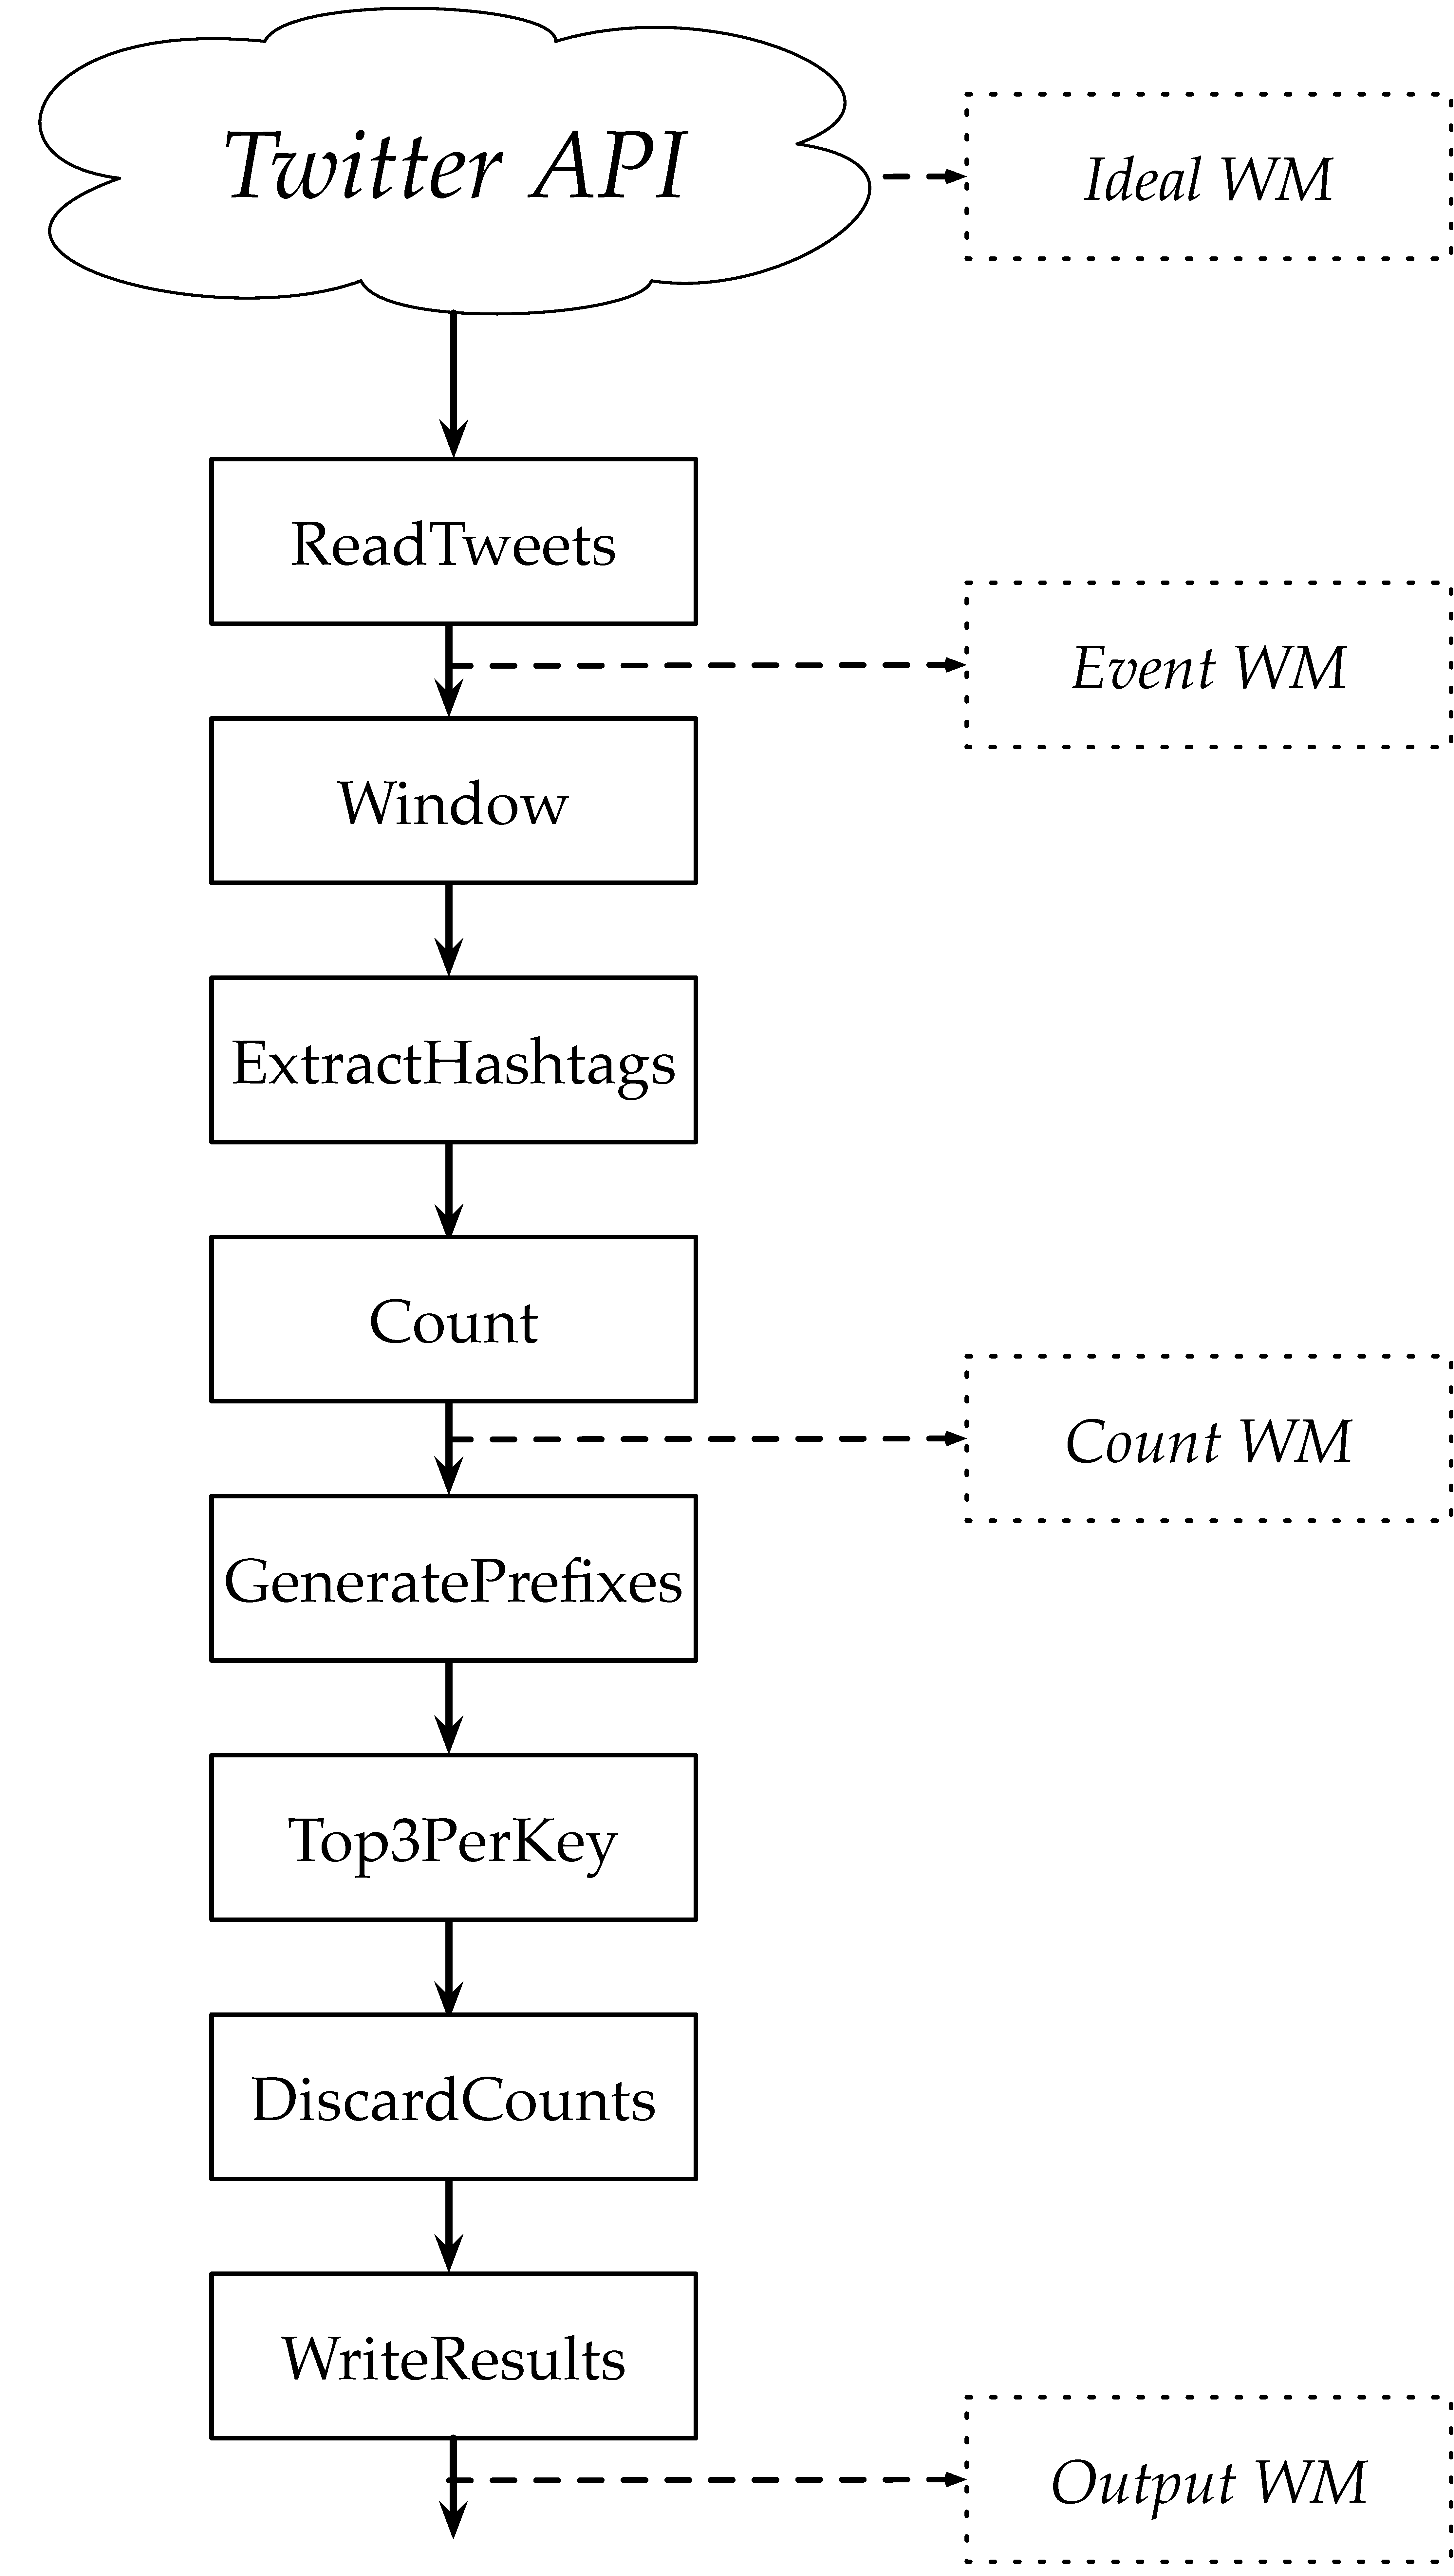
\includegraphics[height=0.6\textheight]{images/diags/eval-twitter-watermarks}
	\caption[The Twitter Pipeline showing the points at which watermarks were measured.]{The Pipeline was instrumented to log the watermark at several points in the Pipeline. The Ideal watermark is not a real measurement. Rather, it is used for comparison.}
	\label{fig:eval:twitter:pipeline-instrument}
\end{figure}


The Pipeline was instrumented to log the watermark at three points, as \cref{fig:eval:twitter:pipeline-instrument} illustrates.
Additionally, CPU and memory usage were collected twice per second.

The goal of the experiment was to find the multiplicative factor $F$ at which the Pipeline could no longer keep up with the stream and produce a pane of output every minute.
It was found that a factor of \num{750}, translating to approximately \num{37500} tweets per second, caused the Pipeline to fall behind.

\subsubsection{Results}

\Cref{fig:eval:twitter:throughput}\subref{fig:eval:twitter:throughput:500} shows the results when $F = 500$.
The Pipeline is keeping up with the stream---the Event and Count watermarks stay almost exactly \SI{30}{\second} behind the true watermark (as per the heuristic used).
The Output watermark indicates that a pane is output every minute---when this happens, a watermark hold is released and the Output watermark can advance to the next window.
The CPU trace shows that mostly two hyperthreads are busy processing data with periods of idleness.
On pane output, a third hyperthread does work, indicated by spikes towards \SI{300}{\percent} CPU usage.

On the other hand, in \cref{fig:eval:twitter:throughput}\subref{fig:eval:twitter:throughput:750} the Pipeline can be seen falling behind when $F = 750$.
The clearest indication of this is the Output watermark---a pane is output every \SI{1.3}{\min}, meaning that each pane becomes more and more out of date with respect to the live data.
It is also evident that the Event watermark is diverging from the Ideal watermark, and the Count watermark is diverging from the Event watermark.
This indicates that both of these Elementwise sections of the Pipeline cannot process elements as fast as they receive them.

The CPU trace offers a hint as to the cause of this---the CPU usage oscillates around \SI{200}{\percent}, with no idle time.
This means that two hyperthreads are executing as fast as possible, even though there are unused hyperthreads.
A common optimisation in other Beam runners is to automatically parallelise Elementwise Transforms in order to increase throughput in cases like this.
Here, the optimisation would likely boost possible throughput by a significant factor.

\subsubsection{Conclusions}

The Pipeline can sustain a processing speed of over \num{25000} tweets per second, over three times the average Twitter Firehose rate.
Keeping in mind that each hashtag in each tweet is exploded into all of its possible prefixes, this is very impressive performance in a real-world scenario.
Several optimisations such as Transform coalescing and auto-parallelisation yet to be implemented have the potential to push the performance even further.

\begin{figure}
	\centering
	\subfloat[][\textbf{Elixir: Twitter Pipeline execution at \pmark\num{25000} tweets per second}\\The Event and Count watermarks remain steady at \SI{30}{\second} behind the Ideal WM. The Output WM indicates that a pane of output is delivered every minute, as required. The CPU trace shows that there are periods where the CPU is idle.]{
		\makebox[\textwidth]{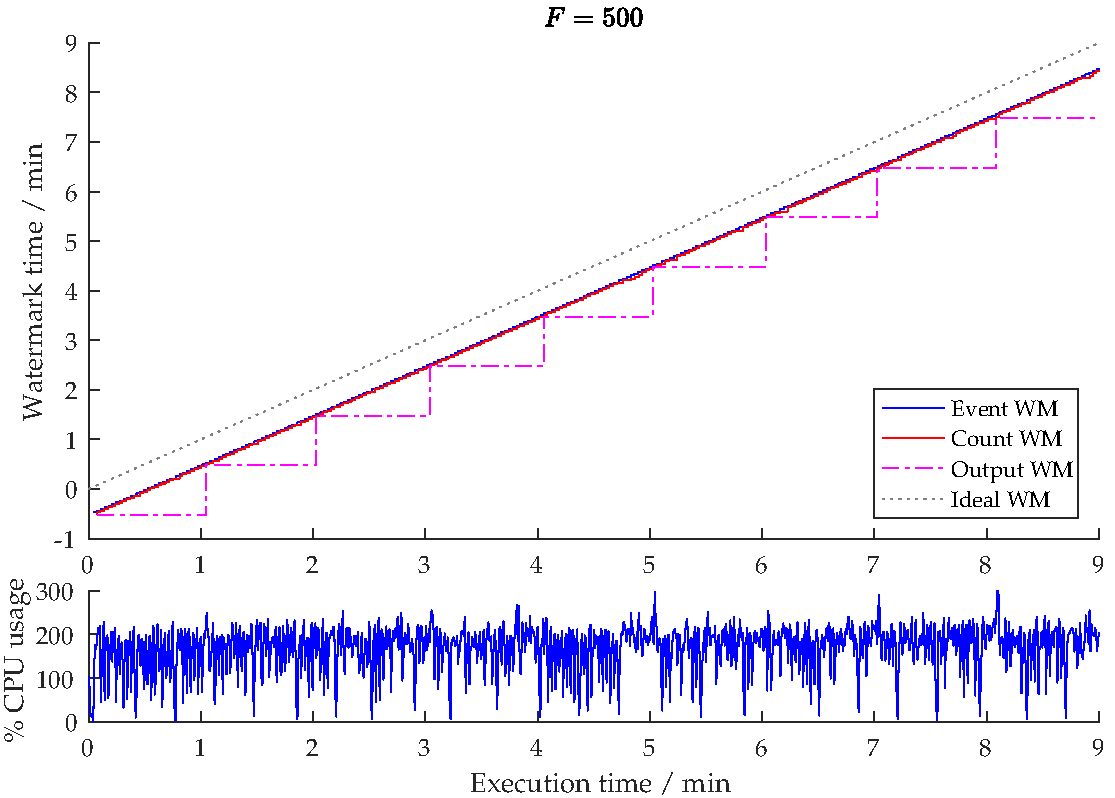
\includegraphics[height=0.41\textheight]{images/graphs/twitter_wm_500}}
		\label{fig:eval:twitter:throughput:500}
	}\\
	\subfloat[][\textbf{Elixir: Twitter Pipeline execution at \pmark\num{37500} tweets per second}\\The Event WM steadily falls behind the Ideal WM, and the Count WM falls behind even further. The Output WM shows output is no longer delivered every minute. The CPU trace shows the code is exhausting two hyperthreads, not able to parallelise further.]{
		\makebox[\textwidth]{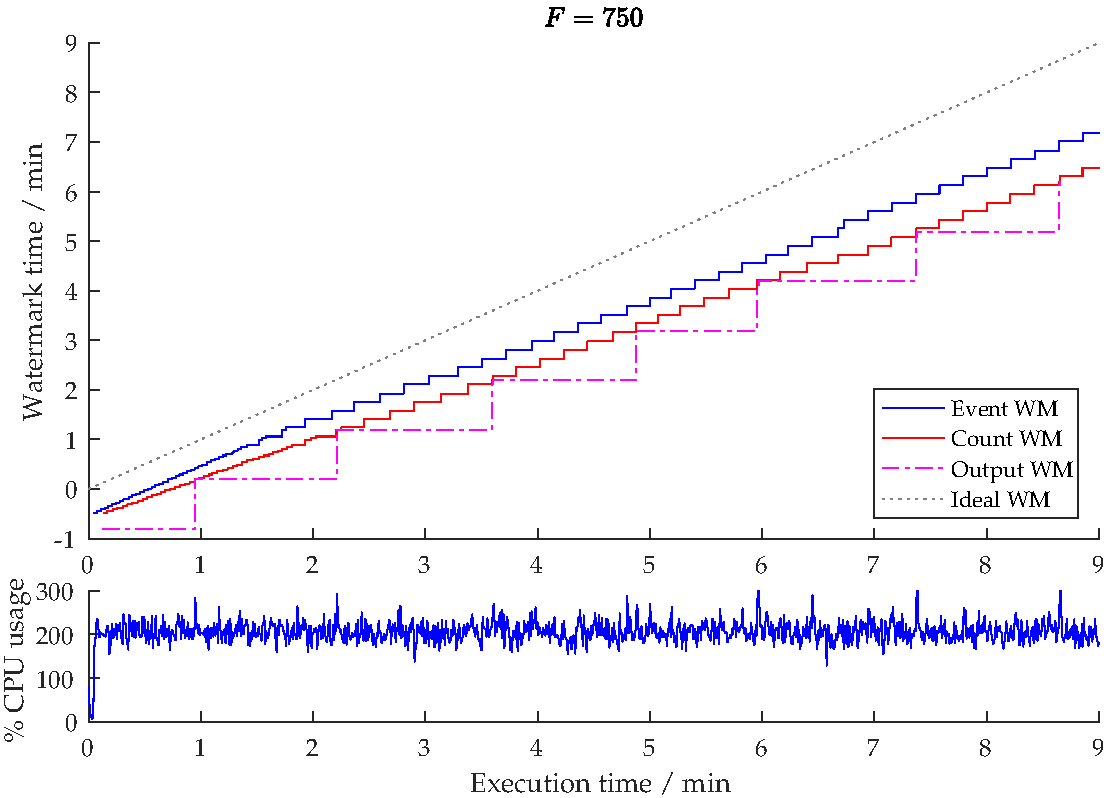
\includegraphics[height=0.41\textheight]{images/graphs/twitter_wm_750}}
		\label{fig:eval:twitter:throughput:750}
	}
	\caption[Watermark and CPU traces of the Elixir runner executing the Twitter Pipeline at two different values of the multiplicative factor.]{The Elixir runner can keep the Twitter Pipeline on time when the multiplicative factor $F$ is \num{500}, but falls behind when it is \num{750}. The CPU usage trace indicates that the bottleneck is the single-threaded execution of Elementwise Transforms.}
	\label{fig:eval:twitter:throughput}
\end{figure}


\section{Latency evaluation}\label{sec:eval:latency}

A key performance indicator of stream-processing systems is the latency of a single element from input to output when the system is under load.
Notwithstanding the Model's powerful windowing features, implementations must display robust streaming performance if they are to subsume existing systems.

\subsection{Methodology}

\begin{figure}
	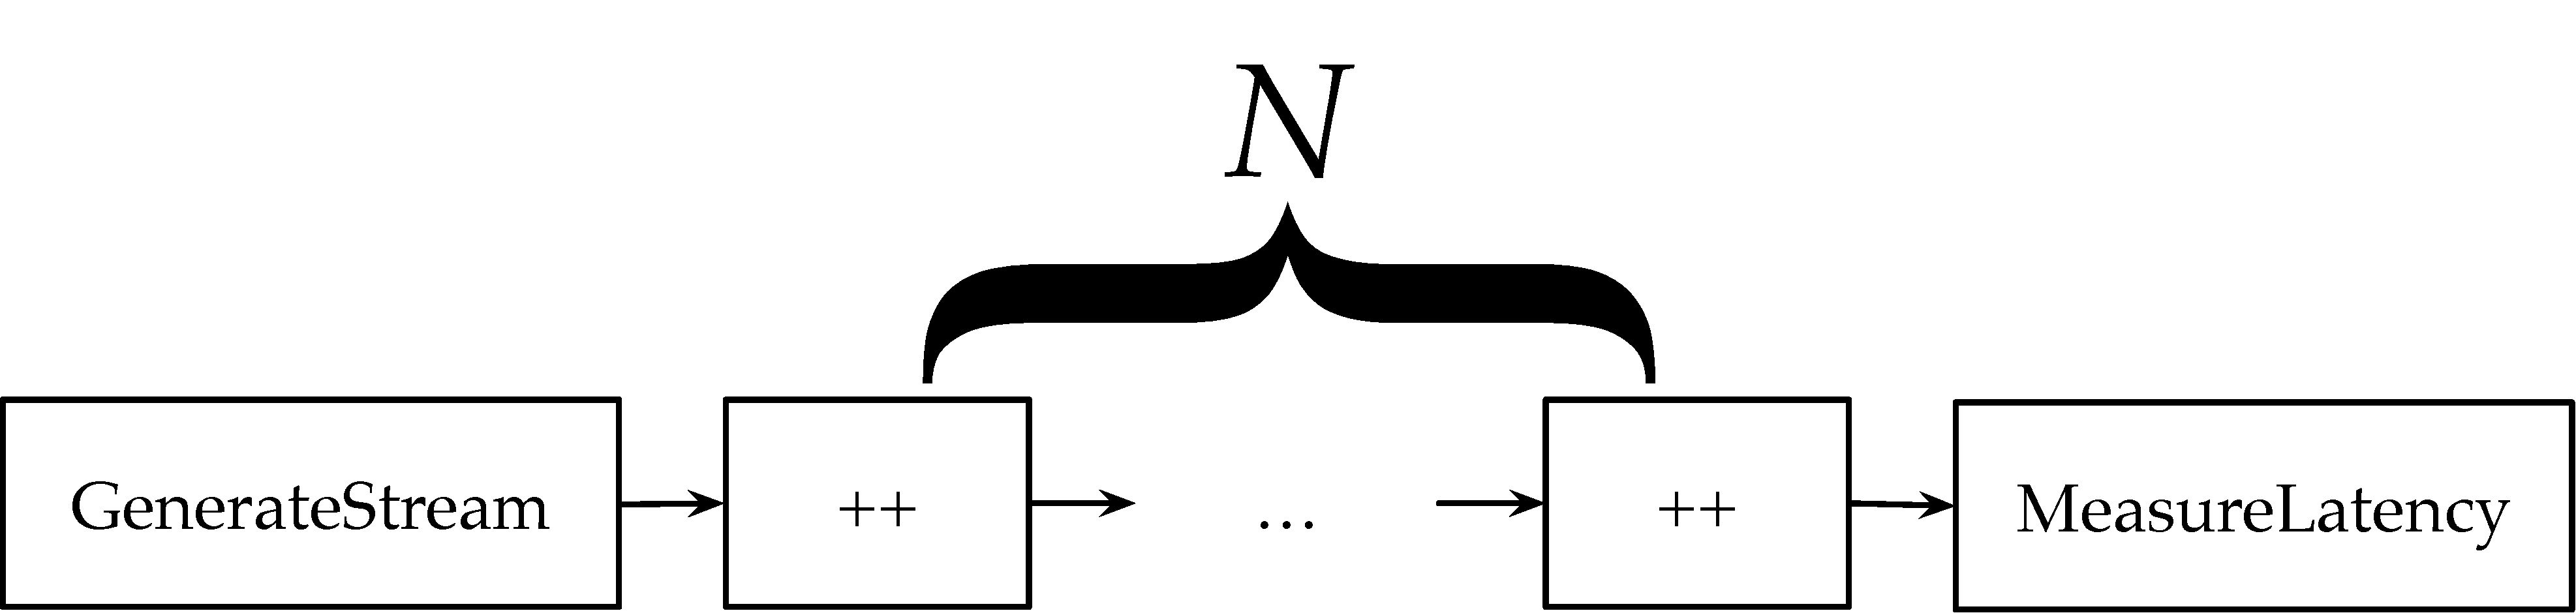
\includegraphics[width=\textwidth]{images/diags/eval-latency-pipeline}
	\caption[The Pipeline used in the latency experiment.]{The Pipeline used to measure latency response to Pipeline length.}
	\label{fig:eval:latency:pipeline-dag}
\end{figure}


In this experiment, a Pipeline was created in which integer elements were generated uniformly at a rate of \SI{100}{\per\second} and passed through a series of \verb|Map| Transforms, each of which incremented the value (\cref{fig:eval:latency:pipeline-dag}).
The latency of each element was measured from the moment of its generation to its output at the last Transform.
The length of the Pipeline was varied and the effects on element latency analysed.
CPU and memory usage were also captured at half-second intervals.

The experiment compared the performance of Elixir Dataflow with the Apache Flink runner, an optimised, production-ready runner for Beam.
The Beam DirectRunner, the default for local Pipelines, was also tested but could not achieve the throughput necessary for its results to be comparable.

Streaming Pipelines tend to be long-running. As such, the first \SI{10}{\second} of data was discarded, as the Java runners showed a large spike in resource usage and element latency while the Pipeline was initialising.
The Elixir runner displayed a similar spike, which was usually shorter than \SI{1}{\second}.

Each instance of the experiment was repeated \num8 times, each time running for \SI{180}{\second}.

\subsection{Runner choice}

The initial experimental design evaluated Pipeline lengths of up to \num{10000} Transforms, comparing the project implementation to the Beam DirectRunner.
However, the DirectRunner ran out of stack space when trying to construct Pipelines longer than $\sim$\num{2000} Transforms.
Given that such large Pipelines are uncommon in practice, the length range was modified to \num{10}--\num{2000} Transforms.

After analysis of the data was carried out, it emerged that the DirectRunner could not in fact handle a \SI{100}{\per\second} stream of elements---the limiting factor was throughput, not latency.
\Cref{fig:eval:latency-graph-java} illustrates the situation.
The element latency grew with time.
This indicates that the runner was falling behind the stream and could not process it in real-time.
This occurred with CPU usage close to \SI{100}{\percent} (even though \num8 hyperthreads were available) and memory usage at \pmark\SI{1.2}{GiB} (even though the heap size was \SI{4}{GB}).
This indicated that the bottleneck was due to the single-threaded design of the runner.
Indeed, it could not even handle a stream of elements at a rate of \SI{10}{\per\second}.

In order to obtain data suitable for a meaningful comparison, the experiment was re-run using the Apache Flink \cite{ApacheFlinkRunner} runner.
The Apache Flink project has focused on implementing the Beam Model and is the production-ready open-source runner most suitable and optimised for execution of Beam Pipelines \cite{ApacheFlinkFocus}.
However, even with the stack size increased to \SI{256}{MB}, it could not construct Pipelines longer than \pmark\num{500} Transforms, and so the range of Pipeline lengths evaluated was reduced.

\begin{figure}
    \centering
	\subfloat[][\textbf{DirectRunner: Element latencies with time at different Pipeline lengths}\\ $N$ is the number of Transforms. Multiple experiment repetitions are shown per plot. The rate of latency growth increases with the Pipeline length.]{
		\makebox[\textwidth]{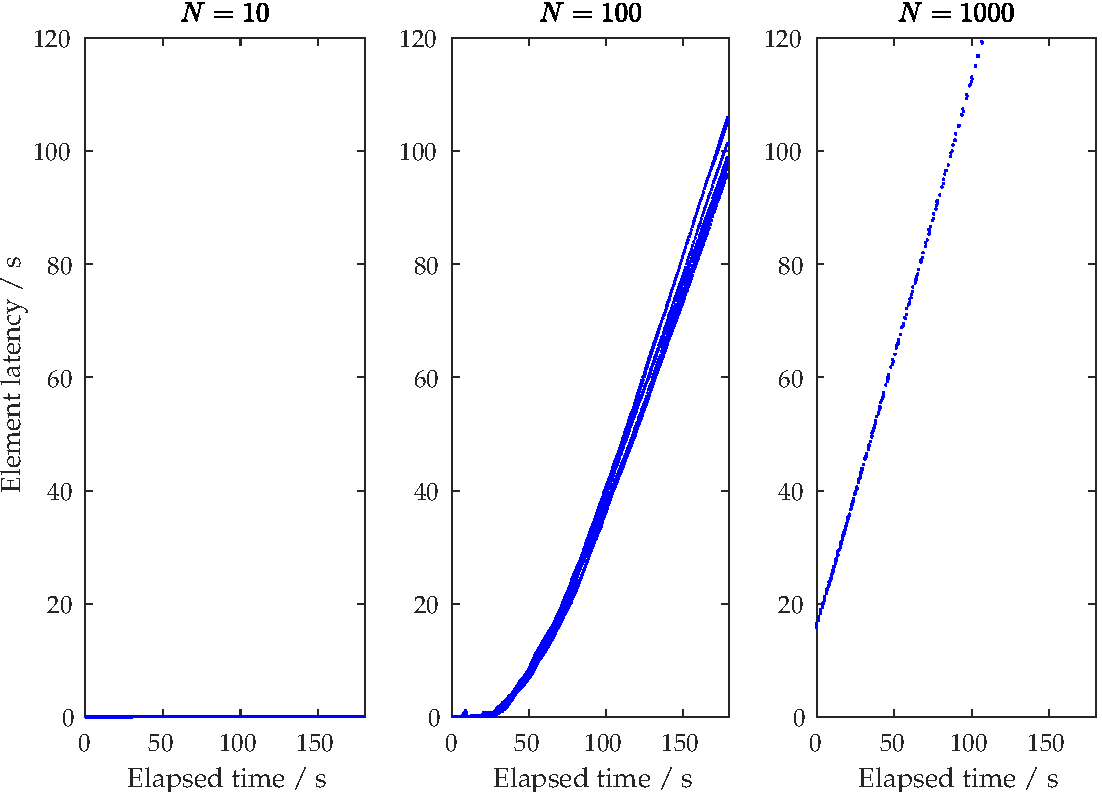
\includegraphics[height=0.42\textheight]{images/graphs/java_latency_demo}}
	}
	
	\subfloat[][\textbf{DirectRunner: CPU and memory usage at different Pipeline lengths}\\The CPU and memory usage remains stable at lengths above \num{100} Transforms. The system does not consume all available resources (\SI{800}{\percent} CPU and \SI{4}{GB} memory).]{
		\makebox[\textwidth]{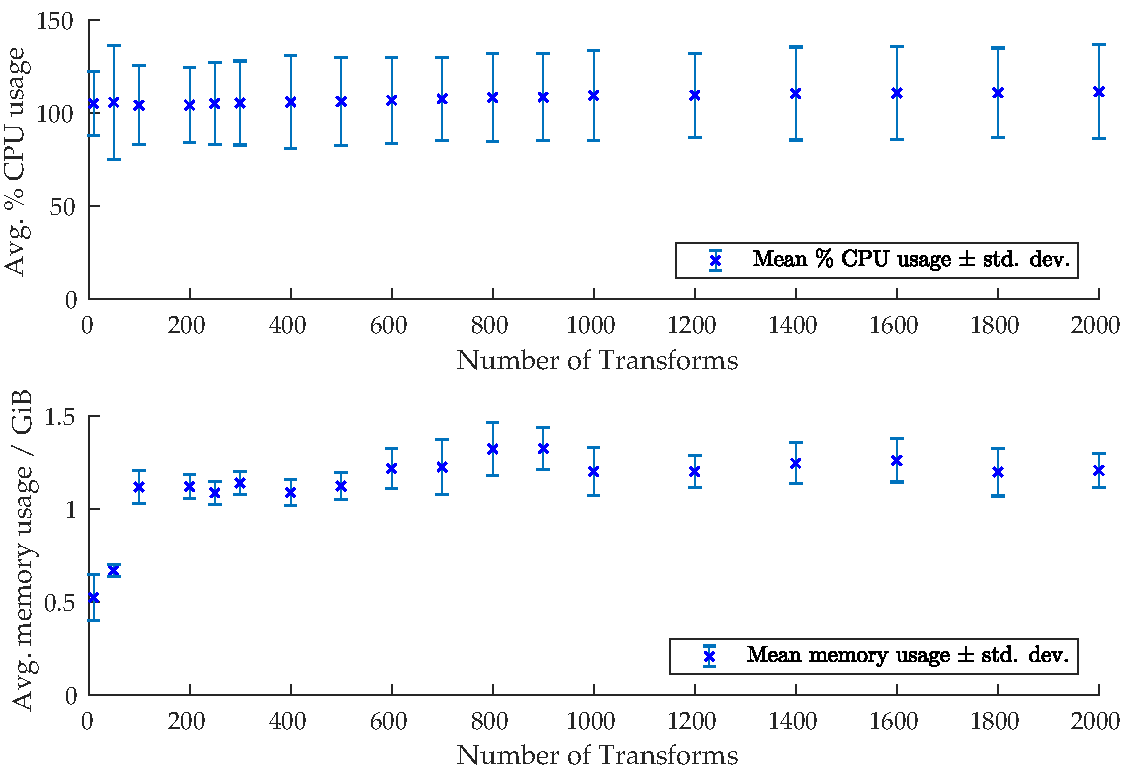
\includegraphics[height=0.42\textheight]{images/graphs/java_memcpu_double}}
	}
	\caption[Results of the latency experiment executed on the DirectRunner, showing its unsuitability.]{The DirectRunner could not maintain sufficient throughput to evaluate the latency of the system under load in a valid way. Data indicate that this is due to the single-threaded design of the runner.}
	\label{fig:eval:latency-graph-java}
\end{figure}

\subsection{Results}

\subsubsection{Latency}

The Elixir runner displayed excellent performance~(\cref{fig:eval:latency-graph-elixir}\subref{fig:eval:latency-graph-elixir:latency}), processing nearly all elements in less than \SI{10}{\milli\second} with a median of \SI8{\milli\second}, even at \num{2000} Transforms.

Both median latency and the inter-quartile range (IQR) increased with Pipeline length, indicating that in longer Pipelines elements experienced increased jitter.
This behaviour is likely due to the randomised scheduling of Transform processes by the BEAM.
The median latency and IQR both remained low (cf. Flink) throughout the range of Pipeline lengths tested, suggesting excellent scalability across that dimension.

The Flink runner exhibited consistent---if unimpressive---latency results~(\cref{fig:eval:latency-graph-flink}\subref{fig:eval:latency-graph-flink:latency}) across the experimental range (which was smaller than that for Elixir).
At all Pipeline lengths, the median latency was \SI{27}{\milli\second} with an IQR of \SI{13}{\milli\second}.
This shows that the runner is able to handle the element stream in this Pipeline length range, but points to a limiting factor.

\subsubsection{Resource consumption}

The Elixir runner displayed CPU usage and memory consumption which scaled linearly with Pipeline length, up to \SI{80}{\percent} and \SI{120}{MiB} at \num{2000} Transforms~(\cref{fig:eval:latency-graph-elixir}\subref{fig:eval:latency-graph-elixir:cpumem}).
There is no indication that either of these resources were a limiting factor.
Instead, it is likely that the runner is prevented from achieving lower latencies by the overhead of switching and I/O between individual processes (Transforms).

The Flink runner also showed a linear trend in its resource consumption~(\cref{fig:eval:latency-graph-flink}\subref{fig:eval:latency-graph-flink:cpumem}).
While its CPU usage was lower than Elixir's in the range tested (by a factor of \num{4}--\num{10}$\times$), its memory usage was significantly higher (by up to \num{60}$\times$) and growing fast with Pipeline length.
This pattern, when viewed against the consistent latency response in \cref{fig:eval:latency-graph-flink}\subref{fig:eval:latency-graph-flink:latency}, paints a picture of a system limited by memory operations like GC and allocation.
The CPU usage is low because the CPU is often waiting around for memory.
This scenario is common in JVM applications.

\subsubsection{Conclusions}

The Elixir runner outperforms Flink with respect to latency across the experimental range, displaying \num{10}--\num{300}$\times$~lower median latency with significantly lower IQR.
It is able to maintain its excellent scalability at Pipeline lengths at which the Flink runner fails to initialise, in spite of not being designed with performance in mind.
This illustrates the power of the BEAM VM to execute concurrent systems in a performant manner while maintaining low resource overheads.

The resource consumption of both runners scales linearly with Pipeline length, though Flink consumes as much as \num{60}$\times$~more memory in spite of lower CPU usage.
In practice, this pattern of memory consumption proves to be a limiting factor much before the CPU usage of Elixir does.

\begin{figure}
    \centering
	\subfloat[Element latency vs.\ Pipeline length.][\textbf{Elixir: Element latency vs.\ Pipeline length} \\An average of \num{128000} elements per box were measured. Each box shows the median and interquartile range. The outlier threshold is $1.5\times$ the IQR. Extreme outliers above \SI{12}{\milli\second} are omitted.]{
		\makebox[\textwidth]{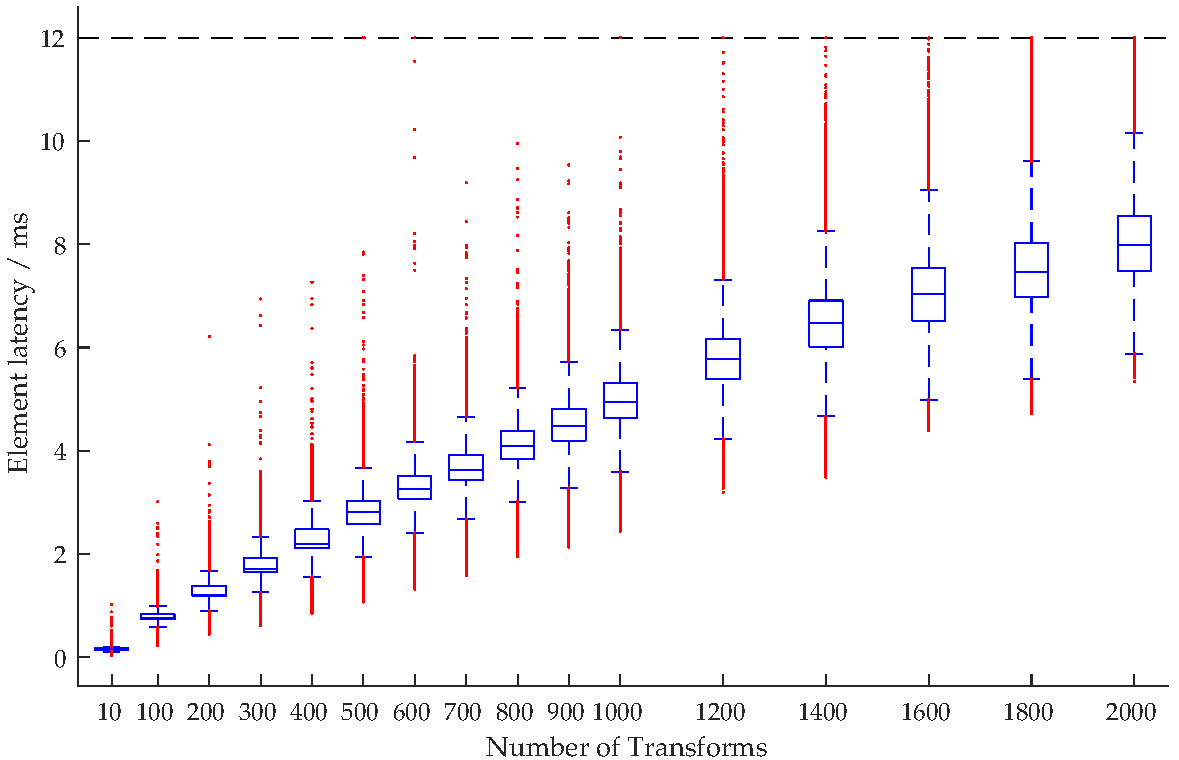
\includegraphics[height=0.42\textheight]{images/graphs/elixir_latency_box}}
		\label{fig:eval:latency-graph-elixir:latency}
	}
	
	\subfloat[Average CPU and memory consumption vs.\ Pipeline length.][\textbf{Elixir: Average CPU and memory consumption vs.\ Pipeline length.} \\ Both resources are consumed with linear growth as the Pipeline length increases, as demonstrated by the good fit of a linear model.]{
		\makebox[\textwidth]{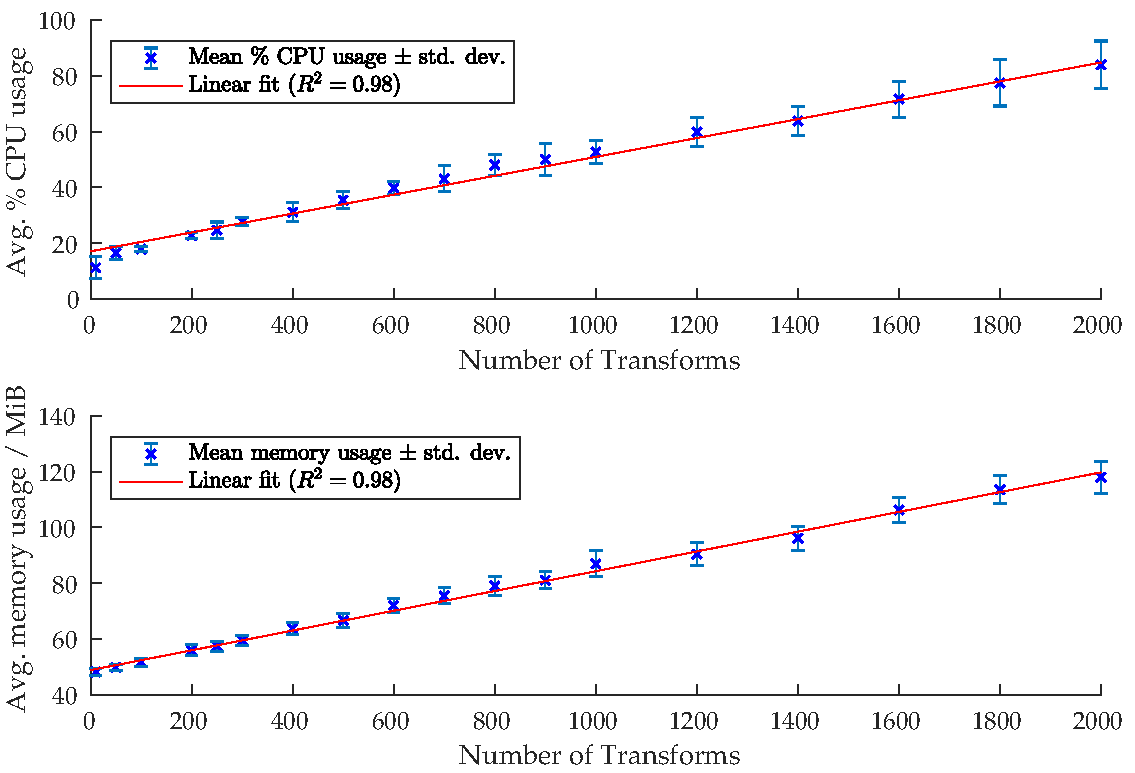
\includegraphics[height=0.42\textheight]{images/graphs/elixir_memcpu_linear}}
		\label{fig:eval:latency-graph-elixir:cpumem}
	}
	\caption[Results of the latency experiment run executed on the Elixir runner.]{The Elixir runner exhibits good scalability under load. When processing elements at a rate of \SI{100}{\per\second}, even very long Pipelines maintain low latency and jitter while maintaining full throughput. Resource consumption scales linearly and predictably with Pipeline length.}
	\label{fig:eval:latency-graph-elixir}
\end{figure}

\begin{figure}
    \centering
	\subfloat[][\textbf{Flink: Element latency vs.\ Pipeline length} \\An average of \num{138000} elements per box were measured. Each box shows the median and interquartile range. The outlier threshold is $1.5\times$ the IQR. Extreme outliers above \SI{80}{\milli\second} are omitted.]{
		\makebox[\textwidth]{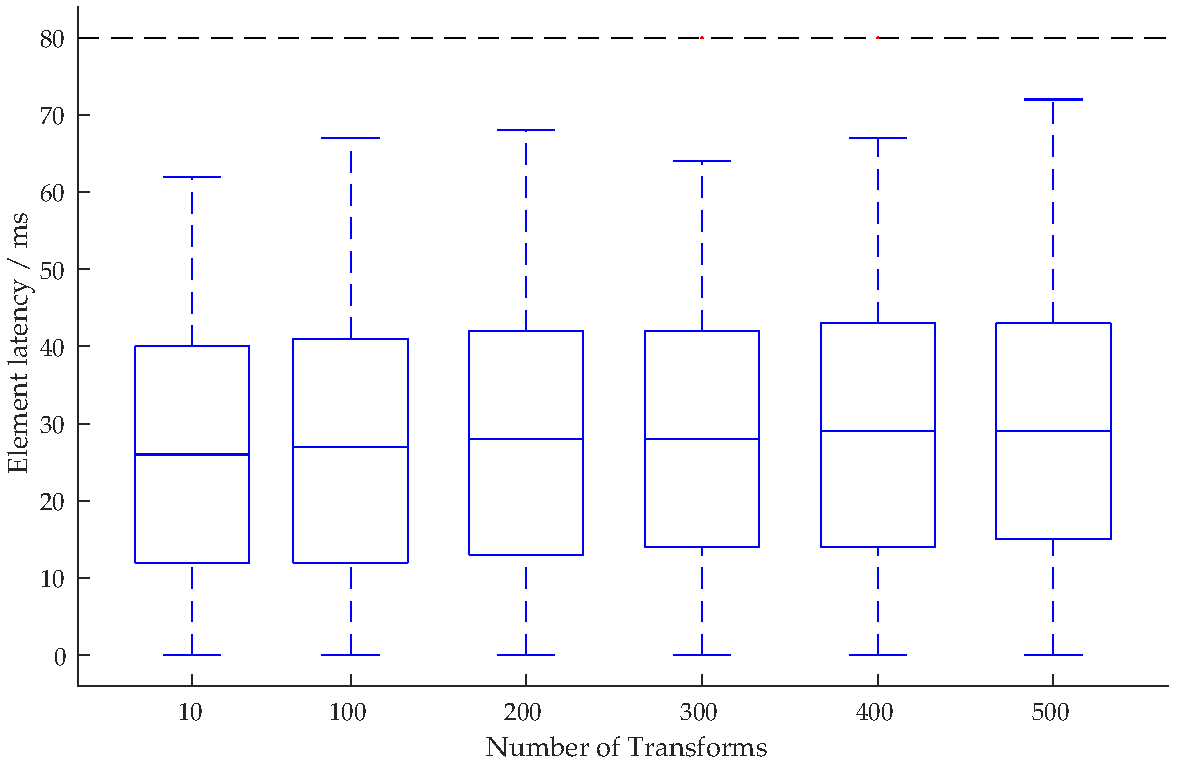
\includegraphics[height=0.42\textheight]{images/graphs/java_flink_latency_box}}
		\label{fig:eval:latency-graph-flink:latency}
	}
	
	\subfloat[][\textbf{Flink: Average CPU and memory consumption vs.\ Pipeline length.} \\ Both resources are consumed with linear growth as the Pipeline length increases, as demonstrated by the good fit of a linear model.]{
		\makebox[\textwidth]{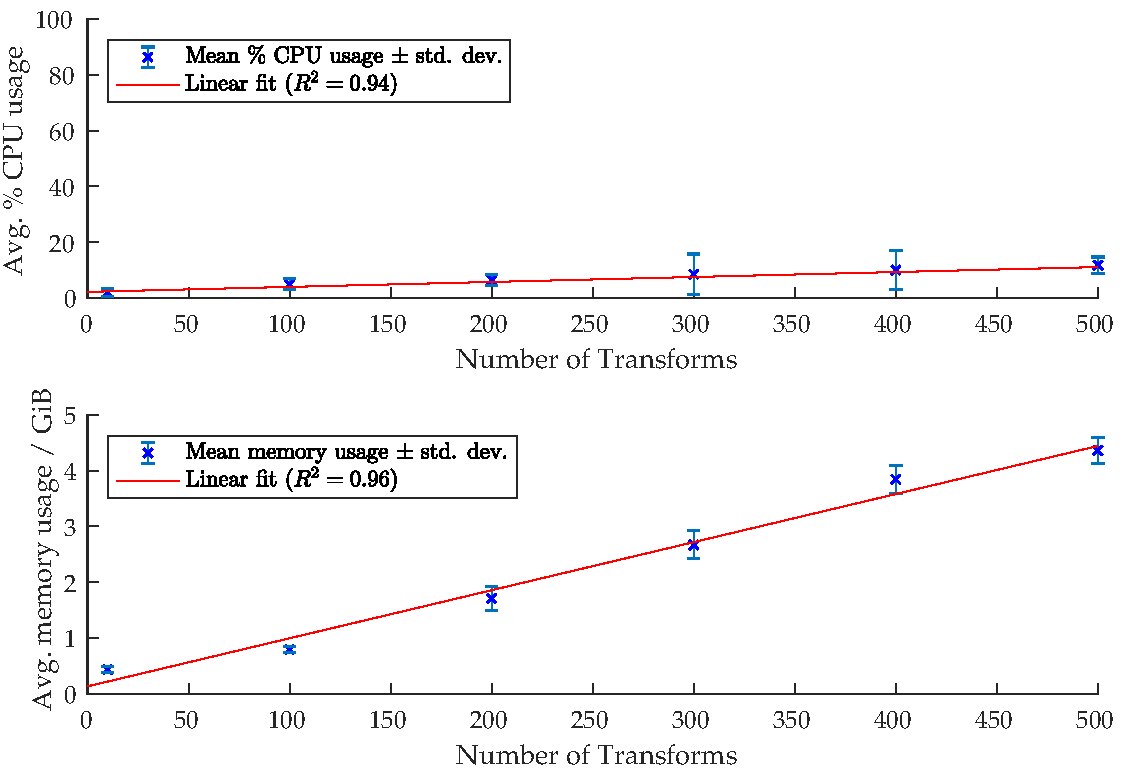
\includegraphics[height=0.42\textheight]{images/graphs/java_flink_memcpu_linear}}
		\label{fig:eval:latency-graph-flink:cpumem}
	}
	\caption[Results of the latency experiment run executed on the Flink runner.]{The Flink runner handles the element stream at full throughput even for longer Pipelines. There is no apparent effect of Pipeline length on element latency in the range tested. Resource consumption scales linearly, but memory usage growth is quite steep even though CPU usage remains low.}
	\label{fig:eval:latency-graph-flink}
\end{figure}
